\FloatBarrier
\section{Questions 1 to 7}
The Matlab implementation of the original system's transfer function is given in \autoref{code:sstr01}. Its step response, shown in \autoref{fig:sstr01}, indicates that the original system is unstable.

\begin{code}
	\begin{matlabcode}{firstnumber = 1}
%% Setting up
clc, clear, close all

%% Required calculations
s = tf('s');
G = 3*(0.4*s+1)*(s+0.8)/((3*s+1)^2*(s+1));
% Settling time
step_info = stepinfo(G);
settling_time = step_info.SettlingTime;
% Sample time
Ts = floor(settling_time)*0.1;

%%  colored noise coefficients
C = [1,0.6,0.4];

%% Original transfer function
G_s = 3*(0.4*s+1)*(s+0.8)/((3*s+1)^2*(s-1));

%% Discrete transfer function
G_discrete = c2d(G_s,Ts,'zoh');
[B,A] = tfdata(G_discrete,'v');
B(1) = [];
	\end{matlabcode}
	\captionof{listing}{Basic system implementation}
	\label{code:sstr01}
\end{code}

\begin{figure}
	\centering
	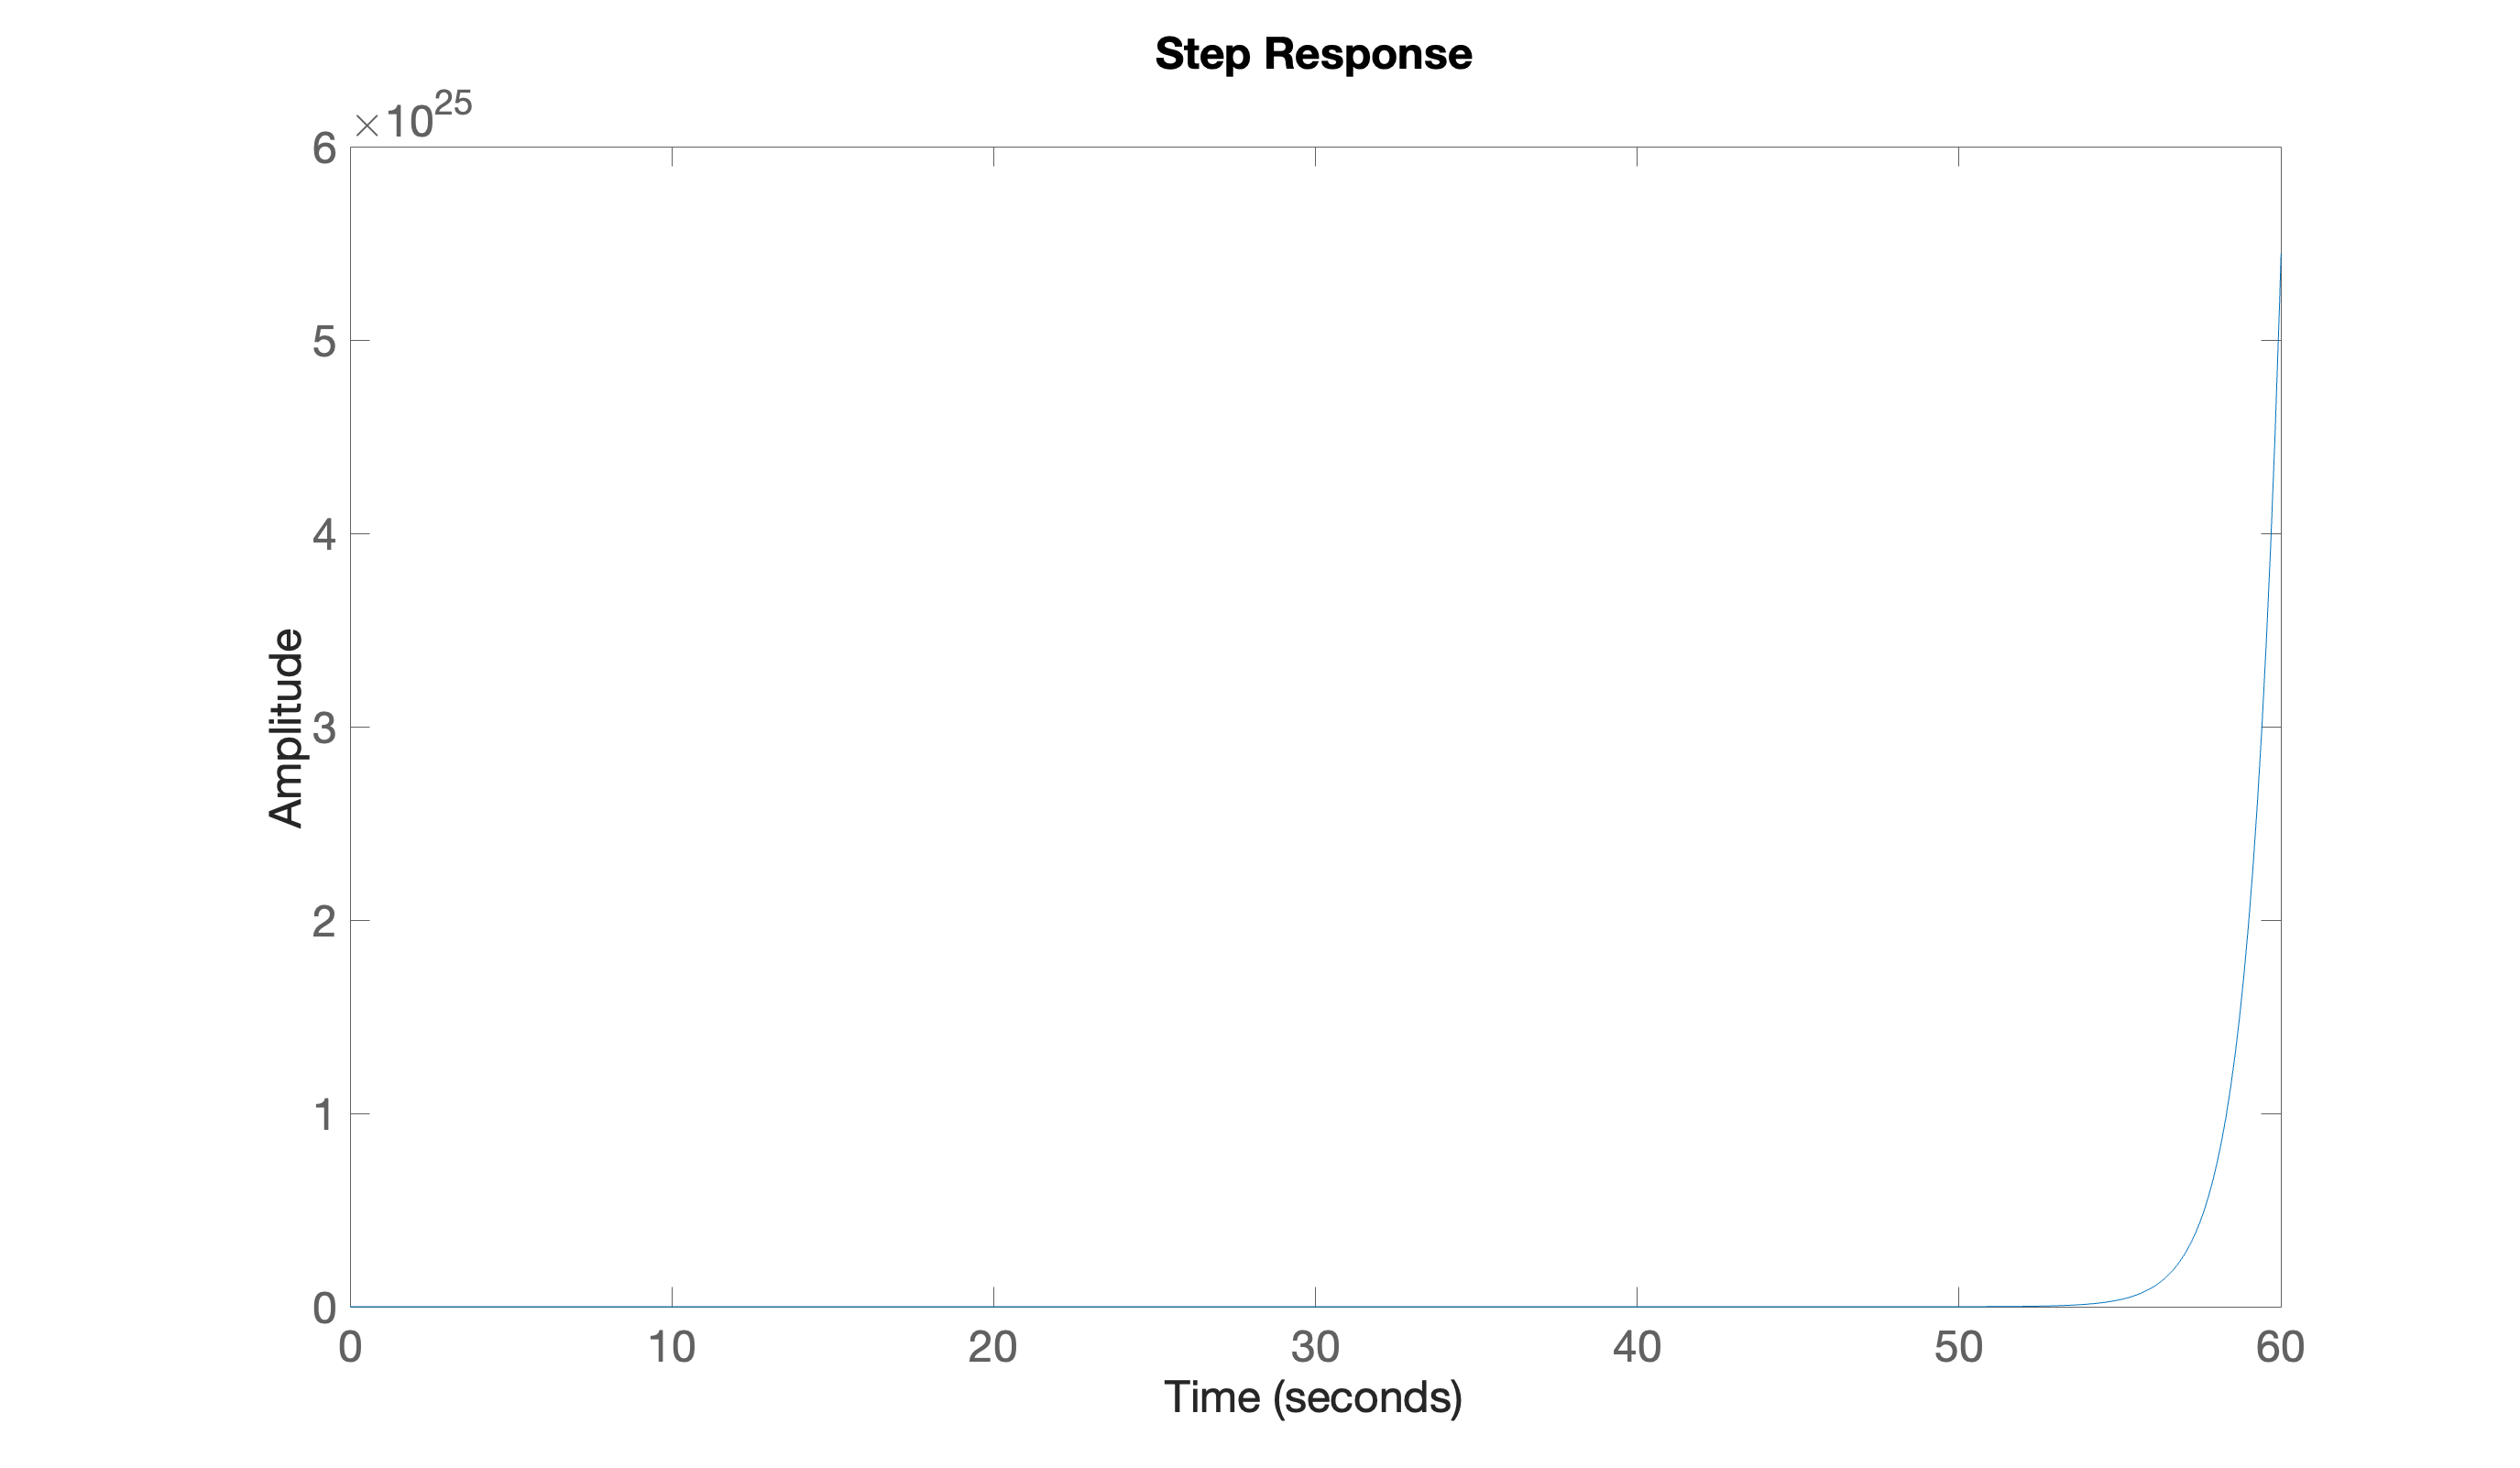
\includegraphics[width=\textwidth]{images/sstr01.png}
	\caption{Original system step response}
	\label{fig:sstr01}
\end{figure}

To enable the calculation of the system's settling time, the unstable pole was mirrored and the system was discretized, as implemented in the code shown in \autoref{code:sstr01}. The step response of the resulting, modified system is presented in \autoref{fig:sstr02}. The system rise time is 9.81 and settling time is 16.71 seconds. 

\begin{figure}
	\centering
	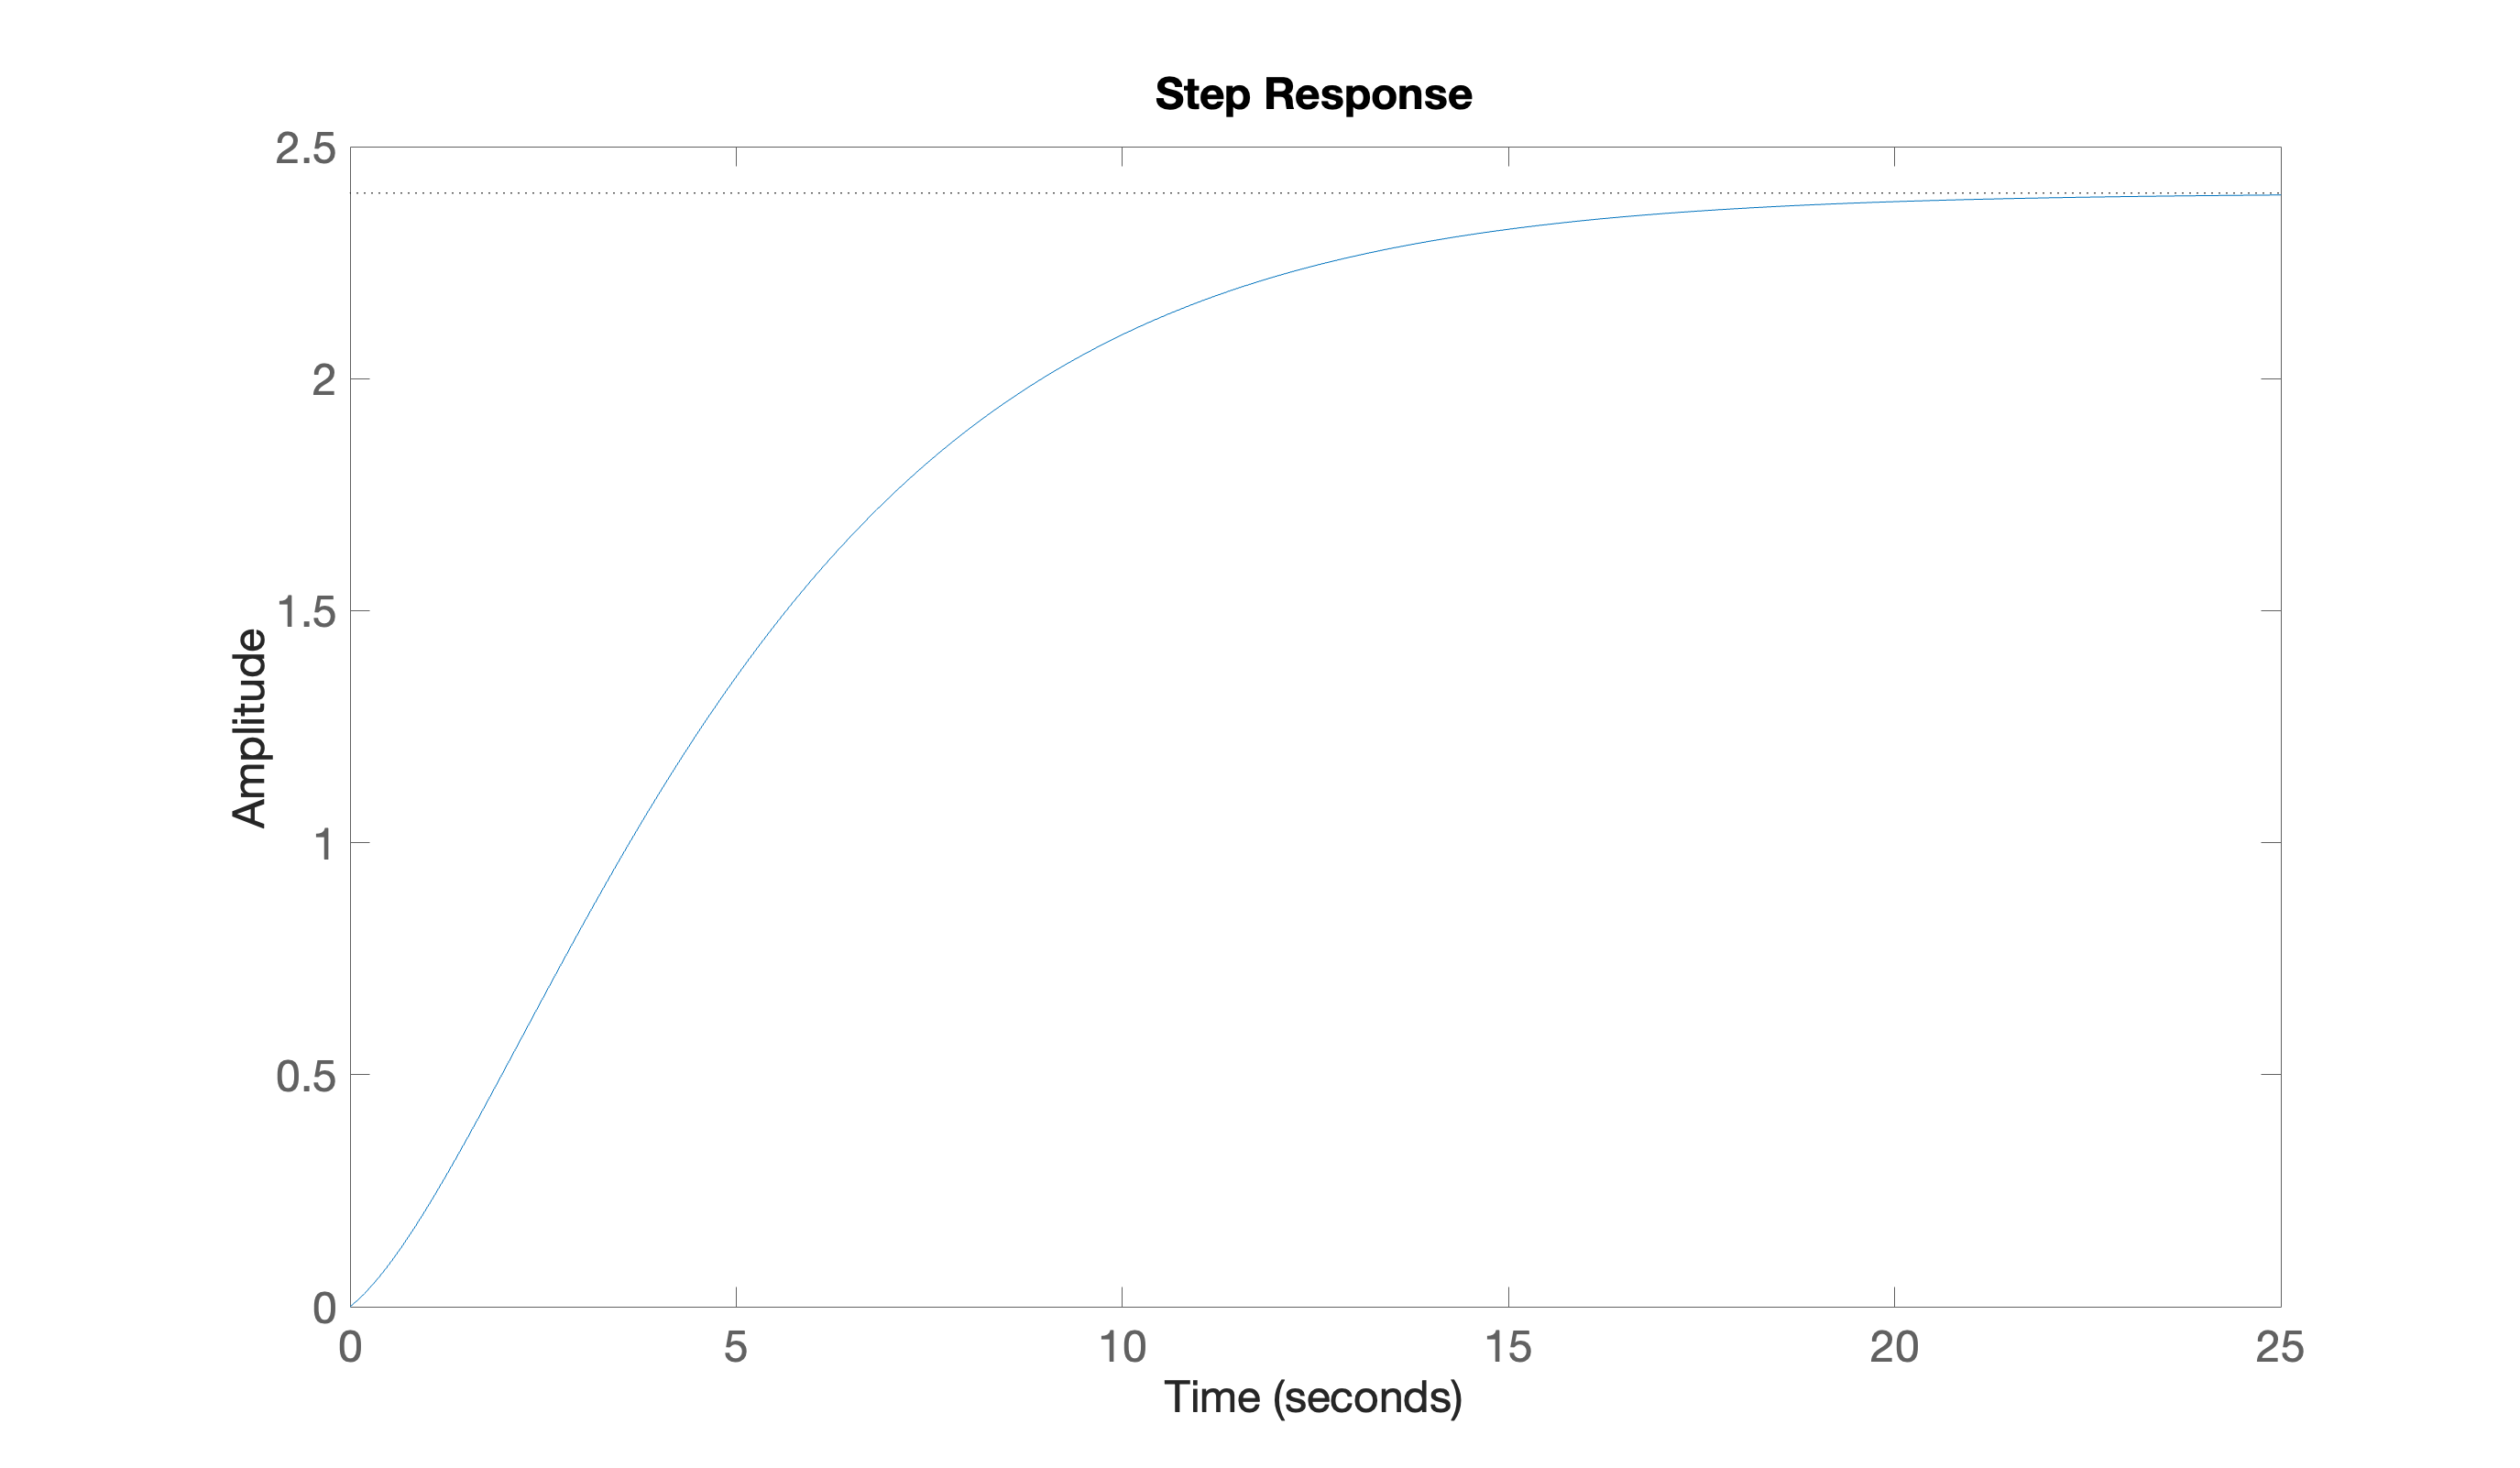
\includegraphics[width=\textwidth]{images/sstr02.png}
	\caption{Discrete stable system step response}
	\label{fig:sstr02}
\end{figure}



\noindent The code for this section is available at \lstinline|assignment3/SSTR/SSTR_0.m|. 


\import{Part1Subsections/}{q1.tex}
\import{Part1Subsections/}{q2.tex}
\import{Part1Subsections/}{q3.tex}
\import{Part1Subsections/}{q4.tex}
\import{Part1Subsections/}{q5.tex}
\import{Part1Subsections/}{q6.tex}
\import{Part1Subsections/}{q7.tex}